% Digital Logic Lab 7
% Created: 2020-03-04, Ashlie Lackey & Megan Gordon

%==========================================================
%=========== Document Setup  ==============================

% Formatting defined by class file
\documentclass[11pt]{article}

% ---- Document formatting ----
\usepackage[margin=1in]{geometry}	% Narrower margins
\usepackage{booktabs}				% Nice formatting of tables
\usepackage{graphicx}				% Ability to include graphics

%\setlength\parindent{0pt}	% Do not indent first line of paragraphs 
\usepackage[parfill]{parskip}		% Line space b/w paragraphs
%	parfill option prevents last line of pgrph from being fully justified

% Parskip package adds too much space around titles, fix with this
\RequirePackage{titlesec}
\titlespacing\section{0pt}{8pt plus 4pt minus 2pt}{3pt plus 2pt minus 2pt}
\titlespacing\subsection{0pt}{4pt plus 4pt minus 2pt}{-2pt plus 2pt minus 2pt}
\titlespacing\subsubsection{0pt}{2pt plus 4pt minus 2pt}{-6pt plus 2pt minus 2pt}

% ---- Hyperlinks ----
\usepackage[colorlinks=true,urlcolor=blue]{hyperref}	% For URL's. Automatically links internal references.

% ---- Code listings ----
\usepackage{listings} 					% Nice code layout and inclusion
\usepackage[usenames,dvipsnames]{xcolor}	% Colors (needs to be defined before using colors)

% Define custom colors for listings
\definecolor{listinggray}{gray}{0.98}		% Listings background color
\definecolor{rulegray}{gray}{0.7}			% Listings rule/frame color

% Style for Verilog
\lstdefinestyle{Verilog}{
	language=Verilog,					% Verilog
	backgroundcolor=\color{listinggray},	% light gray background
	rulecolor=\color{blue}, 			% blue frame lines
	frame=tb,							% lines above & below
	linewidth=\columnwidth, 			% set line width
	basicstyle=\small\ttfamily,	% basic font style that is used for the code	
	breaklines=true, 					% allow breaking across columns/pages
	tabsize=3,							% set tab size
	commentstyle=\color{gray},	% comments in italic 
	stringstyle=\upshape,				% strings are printed in normal font
	showspaces=false,					% don't underscore spaces
}

% How to use: \Verilog[listing_options]{file}
\newcommand{\Verilog}[2][]{%
	\lstinputlisting[style=Verilog,#1]{#2}
}




%======================================================
%=========== Body  ====================================
\begin{document}

\title{ELC 2137 Lab 7: Binary Coded Decimal}
\author{Ashlie Lackey and Megan Gordon}

\maketitle


\section*{Summary}
This lab explored using a Basys3 board to display a number in binary into decimal. Utilizing the double dabble theorem, the input binary numbers were displayed as BCD values. The algorithm started with a basic addition of 3, shift, corresponding to the double-dabble, to convert a 4-bit number. The 3-bit adder was then used also to creat a 6-bit BCD, an 11-bit BCD, and finally, corresponding to the sseg on the Basys3 board. 


\section*{Results}
Below are the ERT's and waveforms of the simulations ran(one for the add3, 6-bit BCD, 11-bit BCD). Along with the expected results tables for every testbench, are pictures of the Basys3 board displaying values for BCD 98 as well as a schematic of the 11-bit Circuit. 


\begin{figure}[ht]\centering
	\begin{tabular}{l|rrrrrrrrrrrrrrrr}
		Time (ns): & 0 & 10 & 20 & 30 & 40 & 50 & 60 & 70 & 80 & 90 & 100 & 110 & 120 & 130 & 140 & 150 \\
		\midrule
		Input num (hex) & 0 & 1 & 2 & 3 & 4 & 5 & 6 & 7 & 8 & 9 & a & b & c & d & e & f \\
		\midrule
		Output out & 0 & 1 & 2 & 3 & 4 & 8 & 9 & a & b & c & d & e & f & 0 & 1 & 2 \\
		\bottomrule
	\end{tabular}\medskip

 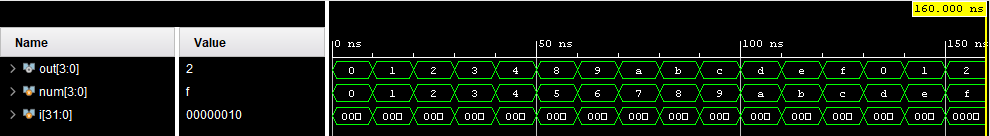
\includegraphics[width=1.1\textwidth]{add3_test.png}
 \caption{add3 Testbench Results}
 \label{fig:sim_with_table}
\end{figure}
\clearpage

\begin{figure}[ht]\centering
	\begin{tabular}{l|rrrrrrr}
		Time (ns): & 0 & 10 & 20 & … & 610 & 620 & 630 \\
		\midrule
		Input (num) & 0 & 1 & 2 & … & 3d & 3e & 3f \\
		\midrule
		Output (out) & 0 & 1 & 2 & … & 61 & 62 & 63 \\
		\bottomrule
	\end{tabular}\medskip

	 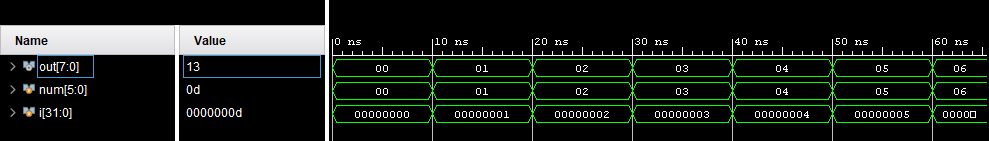
\includegraphics[width=1.1\textwidth]{6bit_test.png}
	 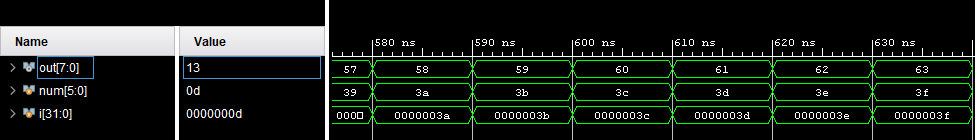
\includegraphics[width=1.1\textwidth]{6bittestend.png}
	 \caption{6bit Testbench Results}
	 \label{fig:6bit Testbench Waveform}

\end{figure}


\begin{figure}[ht]\centering
	\begin{tabular}{l|rrrrrr}
		Time (ns): & 0 & 10 & 20 & 100 & 110 & 120        \\
		\midrule
		Num[10:0] & 000 & 001 & 002 & 061 & 062 & 063      \\
		\midrule
		onest[3:0] & 0 & 1 & 2 & 7 & 8 & 9    \\
		tenst[3:0] & 0 & 0 & 0 & 9 & 9 & 9            \\
		hundredst[3:0] & 0 & 0 & 0 & 0 & 0 & 0 \\
		thousandst[3:0] & 0 & 0 & 0 & 0 & 0 & 0 \\
		
		\bottomrule
		
	\end{tabular}\medskip
	
	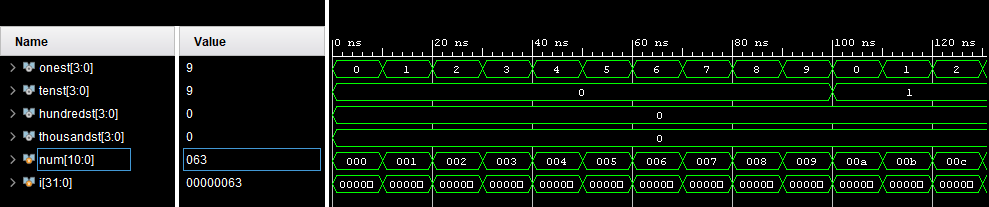
\includegraphics[width=1.1\textwidth]{bcd11_4.png}
	 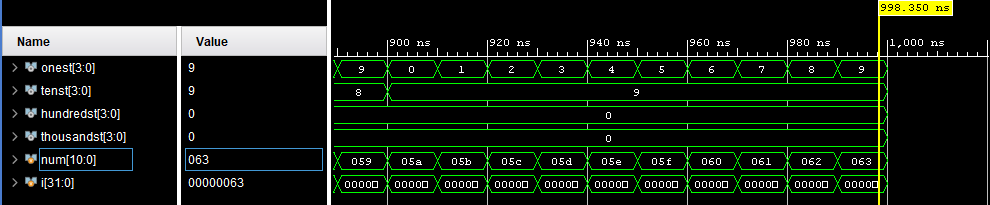
\includegraphics[width=1.1\textwidth]{bcd11_3.png} 
	 \caption{bcd-11 Testbench Results}
	 \label{fig:sim_with_table}
	
\end{figure}

\begin{figure}[ht]\centering
	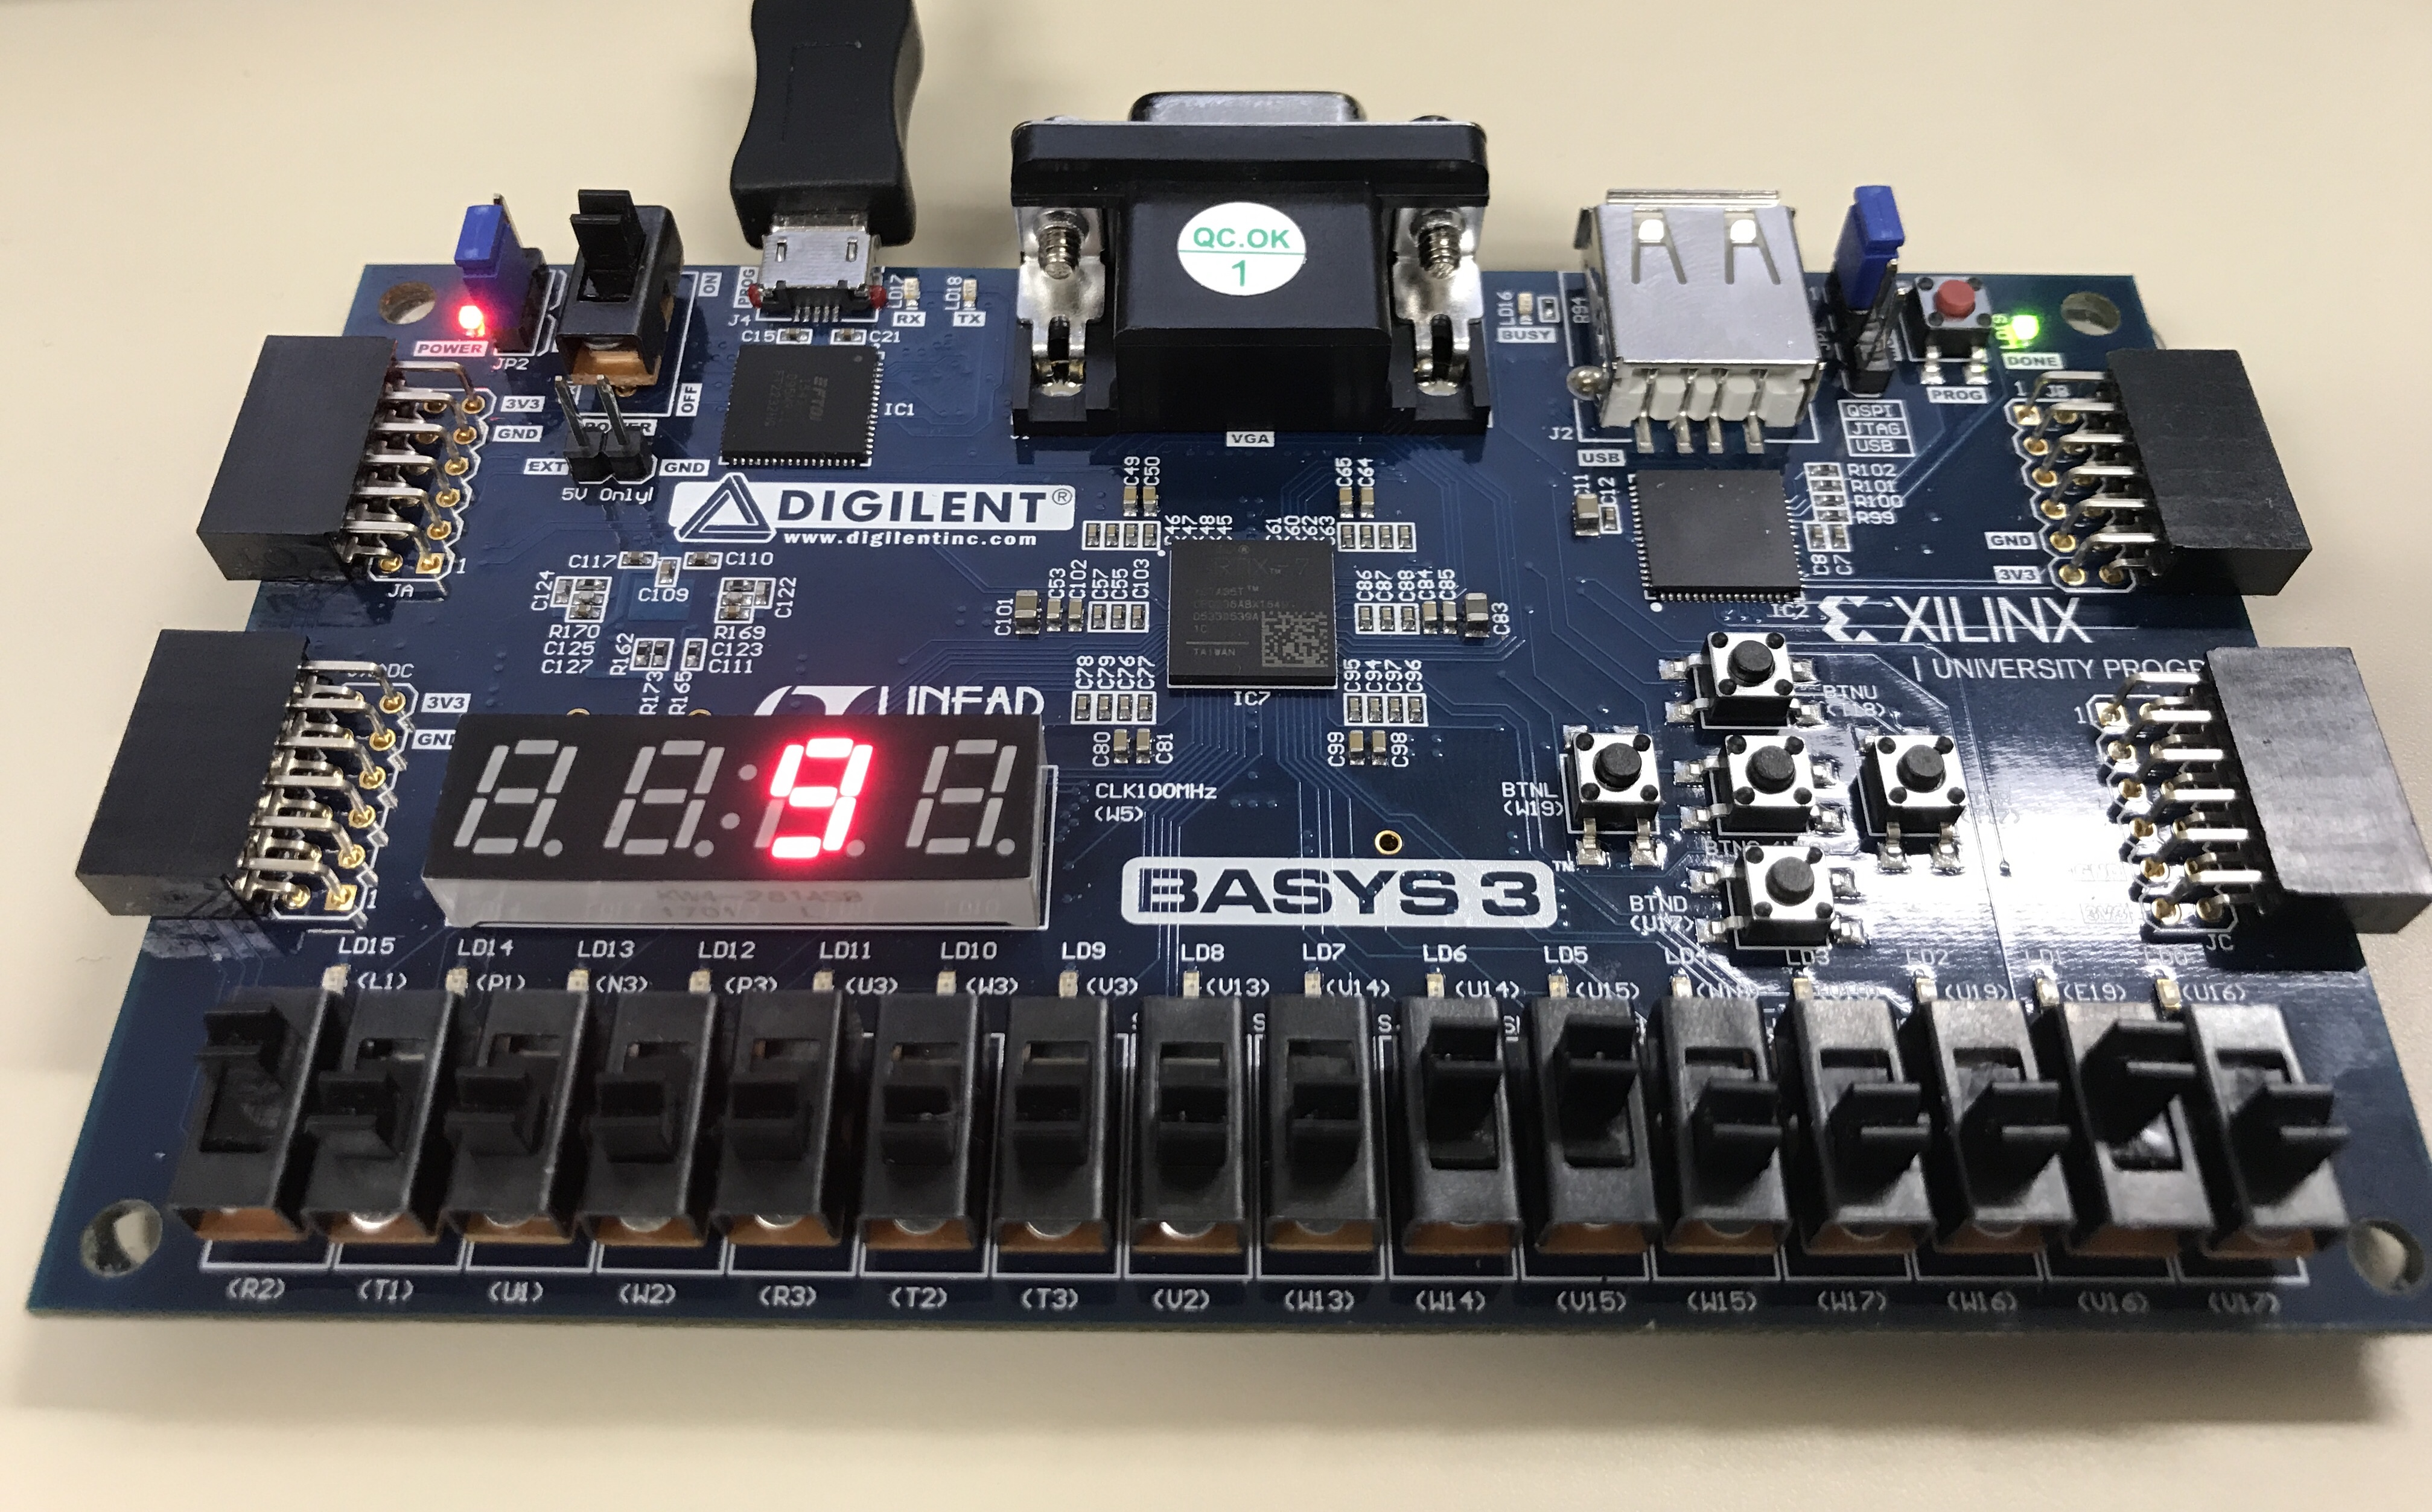
\includegraphics[width=0.65\textwidth]{IMG_1618.jpg}
	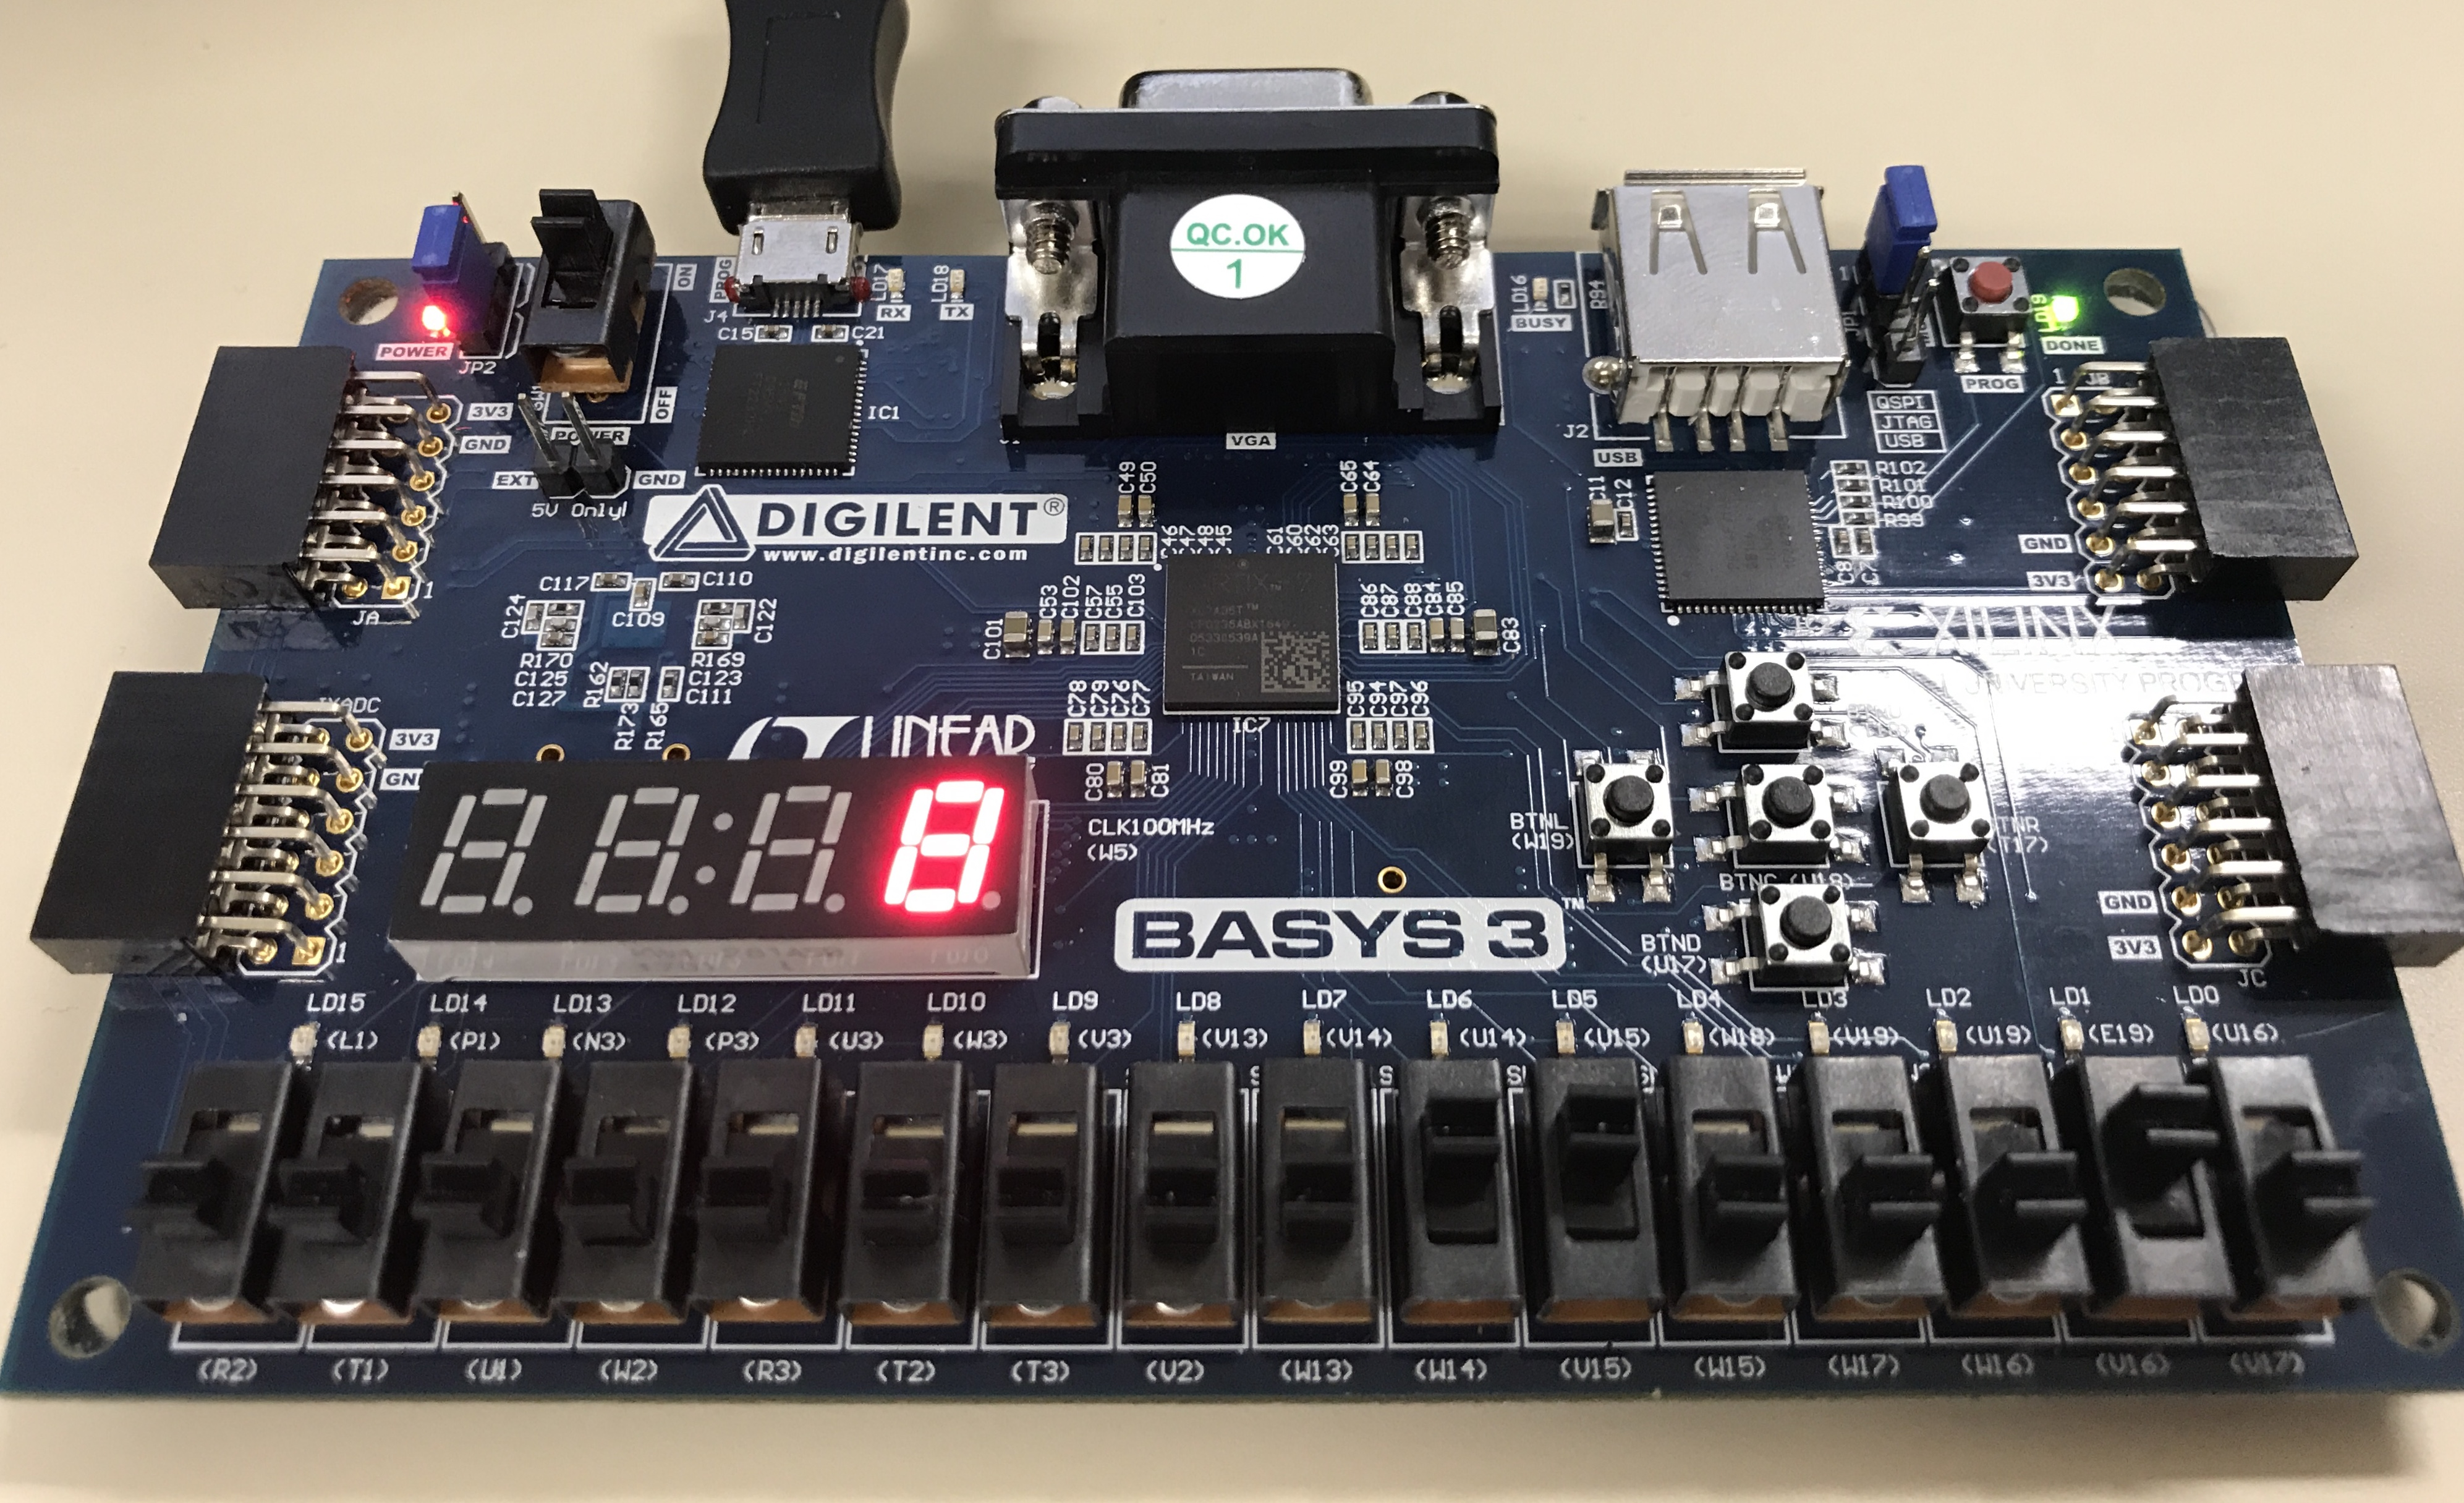
\includegraphics[width=0.65\textwidth]{IMG_1617.jpg}
	\caption{Basys3 BCD Display 98}
	\label{fig:sim_with_table}
	
\end{figure}
\clearpage

\begin{figure}[ht]\centering
	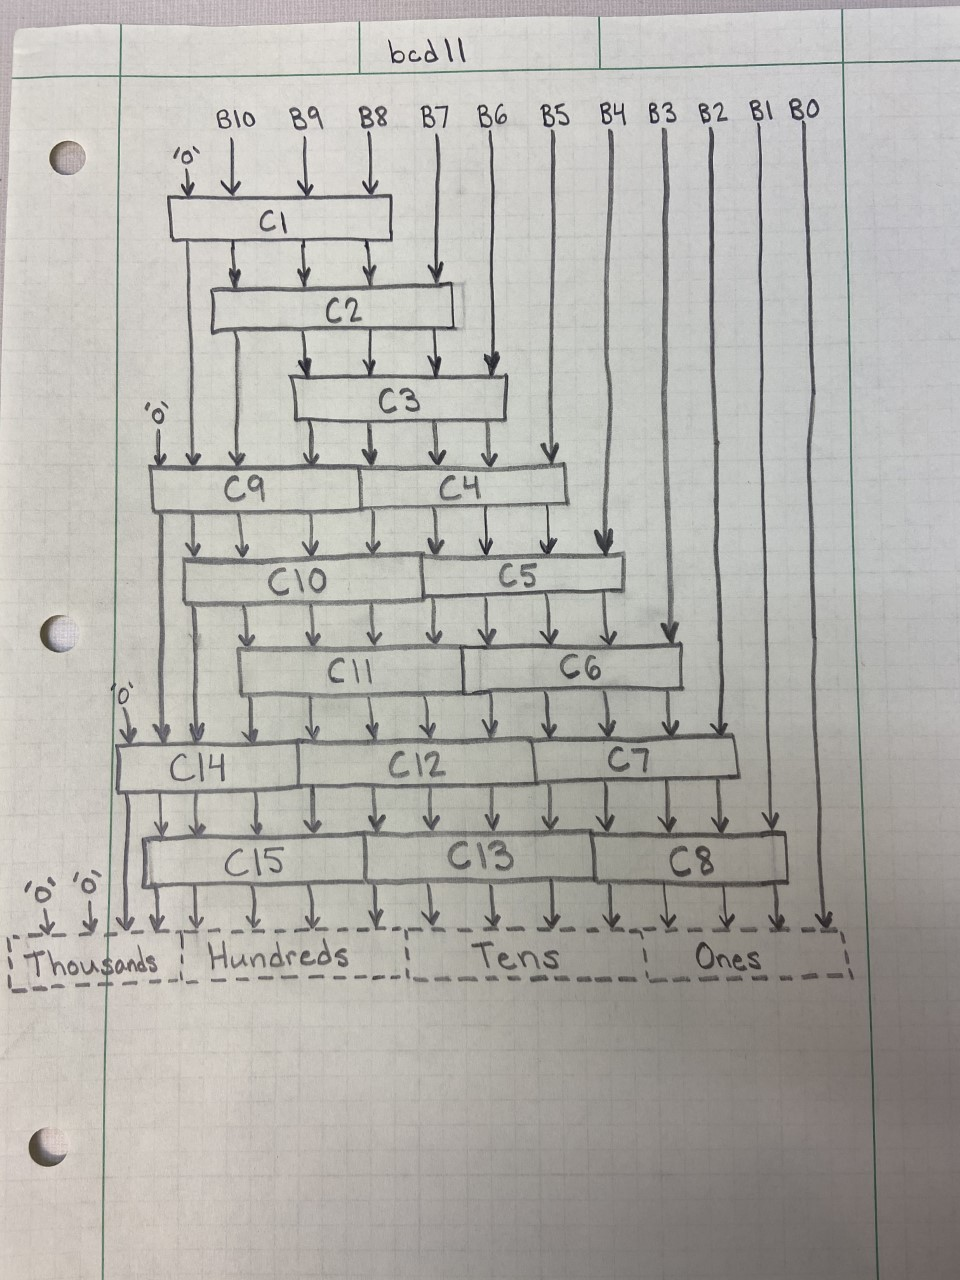
\includegraphics[width=1\textwidth]{bcd11circuit.jpg}
	\caption{}
	\label{fig:sim_with_table}
	
\end{figure}
\clearpage

\section*{Code}
\begin{lstlisting}[style=Verilog,caption=add3 Module Code,label=code:ex ]
`timescale 1ns / 1ps
// Megan and Ashlie, 2137, -02 -27 -2020

module add3(
	input [3:0] B,
	output reg [3:0] Bo
	);
	
	always @*
	if (B > 4'd4)
		Bo = B + 4'd3;
	else
		Bo = B;

endmodule
\end{lstlisting}

\begin{lstlisting}[style=Verilog,caption=6-bit-BCD Module Code,label=code:ex ]
`timescale 1ns / 1ps
// Megan and Ashlie, 2137, -02 -27 -2020

module bit6_BCD(
	input [5:0] Bin,
	output reg [7:0] Bout
	);
	wire [2:0] c12;
	wire [2:0] c23;
	
	add3 c1(.B({0, Bin[5:3]}), .Bo({Bout[6], c12}));
	
	add3 c2(.B({c12, Bin[2]}), .Bo({Bout[5],c23}));
	
	add3 c3(.B({c23, Bin[1]}), .Bo(Bout[4:1]));
	
	assign Bout[7] = 0;
	assign Bout[0] = Bin[0];
endmodule
\end{lstlisting}

\begin{lstlisting}[style=Verilog,caption=bcd11 Module Code,label=code:ex ]
`timescale 1ns / 1ps
// Megan and Ashlie, 2137, -02 -27 -2020
module bcd11(
	input [10:0] B,
	output [3:0] ones, [3:0] tens, [3:0] hundreds, [3:0] thousands);
	
	wire [2:0] c12;
	wire [2:0] c23;
	wire [2:0] c34;
	wire [2:0] c45;
	wire [2:0] c56;
	wire [2:0] c67;
	wire [2:0] c78;
	wire [2:0] c910;
	wire [2:0] c1011;
	wire [2:0] c1112;
	wire [2:0] c1213;
	wire [2:0] c1415;
	wire [11:0] Bout;
	wire [12:0] Bout1;
	
//first left to right(c1-c8)
	add3 ic1(.B({0, B[10:8]}), .Bo({Bout[11], c12}));
	
	add3 ic2(.B({c12, B[7]}), .Bo({Bout[10],c23}));
	
	add3 ic3(.B({c23, B[6]}), .Bo({Bout[9],c34}));
	
	add3 ic4(.B({c34, B[5]}), .Bo({Bout[8], c45}));
	
	add3 ic5(.B({c45, B[4]}), .Bo({Bout[7],c56}));
	
	add3 ic6(.B({c56, B[3]}), .Bo({Bout[6],c67}));
	
	add3 ic7(.B({c67, B[2]}), .Bo({Bout[5],c78}));
	
	add3 ic8(.B({c78, B[1]}), .Bo({tens[0], ones[3:1]}));
//second left to right(c9-c13)
	add3 ic9(.B({0, Bout[11:9]}), .Bo({Bout1[12], c910}));
	
	add3 ic10(.B({c910, Bout[8]}), .Bo({Bout1[11],c1011}));
	
	add3 ic11(.B({c1011, Bout[7]}), .Bo({Bout1[10],c1112}));
	
	add3 ic12(.B({c1112, Bout[6]}), .Bo({Bout1[9],c1213}));
	
	add3 ic13(.B({c1213, Bout[5]}), .Bo({hundreds[0], tens[3:1]}));
//third left to right(c14-c15)
	add3 ic14(.B({0, Bout1[12:10]}), .Bo({thousands[1],c1415}));
	
	add3 ic15(.B({c1415, Bout1[9]}), .Bo({thousands[0], hundreds[3:1]}));
	
	assign thousands[3:2] = 0;
	assign ones[0] = B[0];
endmodule

\end{lstlisting}

\begin{lstlisting}[style=Verilog,caption=sseg1-BCD Module Code,label=code:ex ]
`timescale 1ns / 1ps
// Megan and Ashlie, 2137, -02 -27 -2020
module sseg1_BCD(
	input [15:0]sw,
	output [3:0]an,
	output [6:0]seg,
	output dp
	);
	wire [3:0] uno;
	wire [3:0] diez;
	wire [3:0] cien;
	wire [3:0] mil;
	wire [3:0] keith;
	assign an[1] = ~sw[15];
	assign an[0] = sw[15];
	assign an[3:2] = 2'b11;
	assign dp = 1;
	
	bcd11 terry(.B(sw[10:0]), .ones(uno), .tens(diez), .hundreds(cien), .thousands(mil));
	mux2_4b william (.in1(diez), .in0(uno), .sel(sw[15]), .out(keith));
	sseg_decoder robert(.num(keith), .sseg(seg));
endmodule
\end{lstlisting}

\begin{lstlisting}[style=Verilog,caption=add3-test Testbench Code,label=code:ex ]
`timescale 1ns / 1ps
// Megan and Ashlie, 2137, -02 -27 -2020

module add3_test();
	wire [3:0] out;
	reg [3:0] num;
	integer i;
	
	add3 add3_tester(.B (num), .Bo (out));
	
	initial  begin
		for (i=0; i<=4'hF; i=i+1) begin
			num = i;
			#10;
		end
		$finish;
	end
endmodule
\end{lstlisting}

\begin{lstlisting}[style=Verilog,caption=bit6-BCD-test Testbench Code,label=code:ex ]
module bit6_test();
wire [7:0] out;
reg [5:0] num;
integer i;

bit6_BCD bit6_tester(.Bin(num), .Bout(out));

initial  begin
for (i=0; i<=6'd63; i=i+1) begin
num = i;
#10;
end
$finish;
end
endmodule
\end{lstlisting}

\begin{lstlisting}[style=Verilog,caption=bcd11-test Testbench Code,label=code:ex ]
`timescale 1ns / 1ps
// Megan and Ashlie, 2137, -02 -27 -2020
module bcd11_test();
	wire [3:0] onest, tenst, hundredst, thousandst;
	reg [10:0] num;
	integer i;
	
	bcd11 tester(.B(num), .ones(onest), .tens(tenst), .hundreds(hundredst), .thousands(thousandst));
	
	initial  begin
		for (i=0; i<=11'b11111111111; i=i+1) begin
			num = i;
			#10;
		end
		$finish;
	end
endmodule
\end{lstlisting}

\end{document}